\documentclass[border=2pt]{standalone}
\usepackage{pgfmath}
\usepackage{tikz}
\usetikzlibrary{shapes}
\usetikzlibrary{arrows.meta}
\usetikzlibrary{positioning}
\usetikzlibrary{calc}
\usetikzlibrary{fit}
\usepackage{pgffor}

\renewcommand\familydefault{\sfdefault}
\sffamily

\tikzset{
  arrow/.style = {
    -Latex,
    rounded corners=3mm
  },
  pics/state/.style args = {#1/#2}{
    code = {
      \begin{scope}[yshift=1.5cm]
        \node [anchor=north east] (-label) at (3cm,0cm) {#1};
        \path let \p1 = (-label.south)
              in coordinate (tmp) at (0cm, \y1);

        % invert list
        \let\mylist\empty
        \foreach\x in {#2} {
          \ifx\mylist\empty
            \xdef\mylist{\x}%
          \else
            \xdef\mylist{\x,\mylist}%
          \fi
        }

        \coordinate (tmp) at (0cm,-2cm);

        \foreach[count=\i] \argtext in \mylist {
          \node [inner sep=1pt,anchor=south west] (-\i) at (tmp) {\footnotesize \argtext\phantom{Iq}};
          \path let \p1 = (-\i.north)
            in coordinate (tmp) at (0cm, \y1);
        }

        \node [rectangle,draw,fit={(0cm,0cm) (3cm,-2cm)},inner sep=0pt] (#1) {};
      \end{scope}
    }
  },
}

\begin{document}
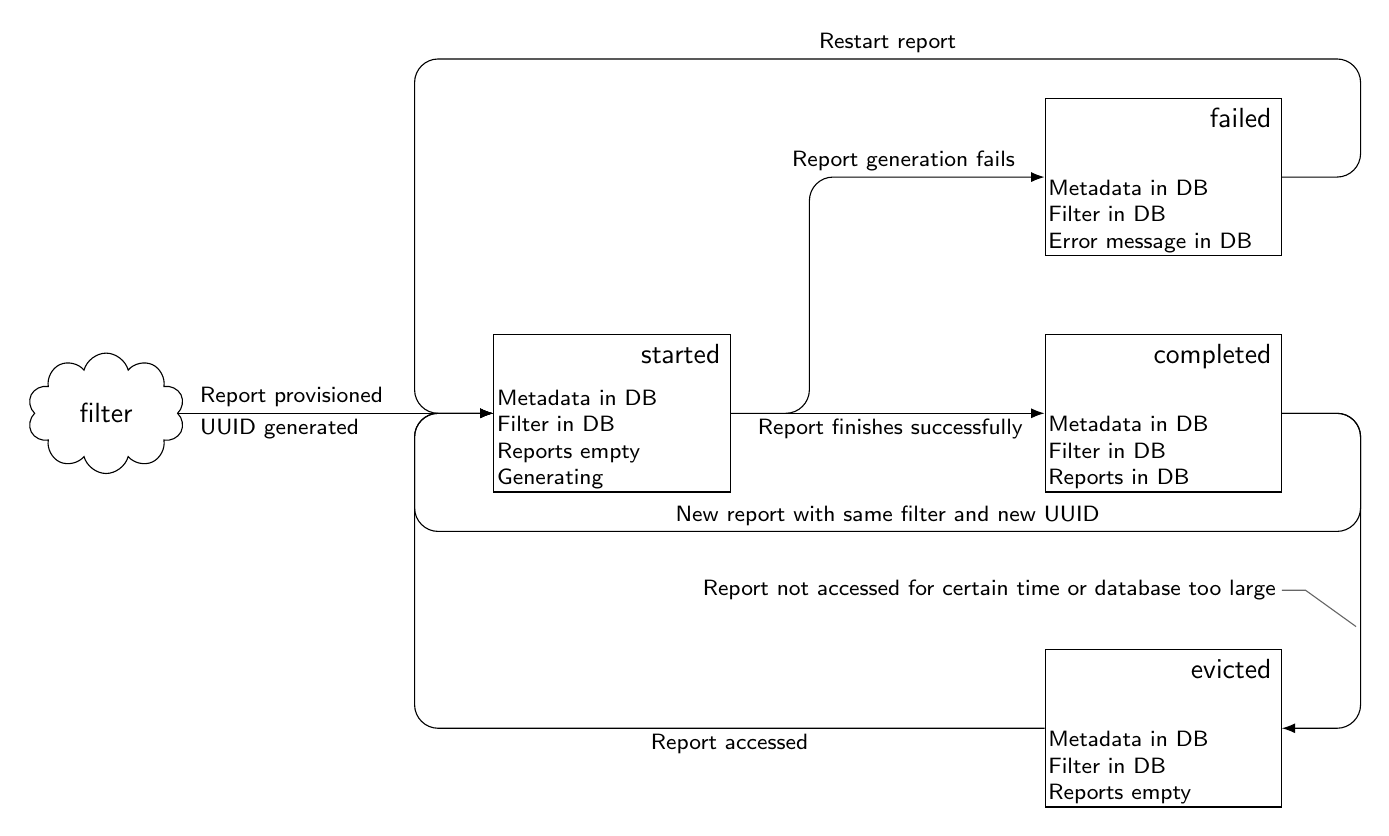
\begin{tikzpicture}
  \pic at (0,0) {state=started/{{Metadata in DB},{Filter in DB},{Reports empty},{Generating}}};
  \pic at (7cm,0) {state=completed/{{Metadata in DB},{Filter in DB},{Reports in DB}}};
  \pic at (7cm,3cm) {state=failed/{{Metadata in DB},{Filter in DB},{Error message in DB}}};
  \pic at (7cm,-4cm) {state=evicted/{{Metadata in DB},{Filter in DB},{Reports empty}}};
  \node [minimum width=2cm,minimum height=1cm,draw,cloud,anchor=east] at ($ (started.west) - (4cm,0) $) (filter) { filter };

  \draw [arrow] (filter.east) -- (started.west)
    node [pos=.05,anchor=south west,inner sep=2pt] {\footnotesize Report provisioned}
    node [pos=.05,anchor=north west,inner sep=2pt] {\footnotesize UUID generated};
  \draw [arrow] (started.east) -- (completed.west)
    node [pos=.95,anchor=north east,inner sep=2pt] {\footnotesize Report finishes successfully};

  \draw [arrow] (completed.east) -- ++(1cm,0) coordinate (evicted-node-first) |- (evicted.east);

  \draw [arrow] (evicted.west) -| ($ (started.west) - (1cm,0) $) coordinate (before-started) -- (started.west);
  \path let \p1 = (evicted.west),
            \p2 = (before-started)
    in node [anchor=north,inner sep=2pt] at ($ (\x1, \y1)!0.5!(\x2,\y1) $) {\footnotesize Report accessed};

  \draw [arrow] (started.east) -- ++(1cm,0) |- (failed.west)
    node [pos=.95,anchor=south east,inner sep=2pt] {\footnotesize Report generation fails};

  \draw [arrow] (failed.east) -| ++(1cm,1.5cm) coordinate (tmp) -| (before-started) -- (started.west);
  \path let \p1 = (tmp),
            \p2 = (before-started)
    in node [anchor=south,inner sep=2pt] at ($ (\x1, \y1)!0.5!(\x2,\y1) $) {\footnotesize Restart report};

  \draw [arrow] (completed.east) -| ++(1cm,-1.5cm) coordinate (tmp) -| (before-started) -- (started.west);
  \path let \p1 = (tmp),
            \p2 = (before-started)
    in node [anchor=south,inner sep=2pt] at ($ (\x1, \y1)!0.5!(\x2,\y1) $) {\footnotesize New report with same filter and new UUID};


  \path let \p1 = (evicted-node-first),
            \p2 = (evicted.east),
            \p3 = (evicted.north),
            \p4 = (tmp)
    in node [inner sep=2pt,anchor=east] (evictlabel) at ($ (\x2,\y4)!0.5!(\x2,\y3) $) {\footnotesize Report not accessed for certain time or database too large}
    coordinate (evictarrow) at ($ (\x4,\y4)!0.5!(\x4,\y2) $);

  \draw [thin,draw=black!60,shorten >=2pt] (evictlabel.east) -- ++(0.3cm,0) -- (evictarrow);
\end{tikzpicture}
\end{document}
